\documentclass[tikz,border=6pt]{standalone}
\usepackage{amsmath,amssymb,bm}
\usepackage{tikz}
\usetikzlibrary{arrows.meta,calc,positioning,fit,backgrounds,decorations.pathreplacing,shapes.geometric,quotes}
\definecolor{okBlue}{HTML}{4472C4}
\definecolor{okRed}{HTML}{C0504D}
\definecolor{okGreen}{HTML}{55A868}
\definecolor{okOrange}{HTML}{D98E04}
\definecolor{okPurple}{HTML}{7E57C2}
\definecolor{okGray}{HTML}{666666}
\definecolor{softBlue}{HTML}{EAF1FB}
\definecolor{softRed}{HTML}{F9ECEB}
\definecolor{softGreen}{HTML}{EDF7F0}
\tikzset{
  >={Latex[length=2.2mm,width=2.0mm]},
  every node/.style={font=\small},
  mathbox/.style={draw=black!55, rounded corners=2pt, very thick, fill=black!2, inner sep=5pt, align=center},
  chip/.style={draw=black!45, rounded corners=1.6pt, fill=black!1, inner sep=2pt, align=center},
  panel/.style={draw=black!55, rounded corners=2pt, line width=0.8pt},
  lightpanel/.style={draw=black!25, rounded corners=2pt, line width=0.5pt},
  flow/.style={-{Latex[length=2.3mm]}, line width=1.0pt, draw=black!70},
  thinflow/.style={-{Latex[length=1.9mm]}, line width=0.8pt, draw=black!55},
  faintcol/.style={draw=black!18, line width=0.6pt},
  reglabel/.style={font=\normalsize},
  srcA/.style={circle, draw=okBlue!70!black, fill=okBlue!15, minimum size=5.2pt, inner sep=0pt},
  srcB/.style={circle, draw=okRed!70!black, fill=okRed!15, minimum size=5.2pt, inner sep=0pt},
  tgtA/.style={circle, draw=okBlue!70!black, fill=okBlue!15, minimum size=5.2pt, inner sep=0pt},
  tgtB/.style={circle, draw=okRed!70!black, fill=okRed!15, minimum size=5.2pt, inner sep=0pt},
  crossdot/.style={diamond, draw=okOrange!80!black, fill=okOrange!85, minimum size=6pt, inner sep=0pt},
  kedge/.style={draw=okBlue!60!black, line width=0.9pt, opacity=0.50},
  triangleedge/.style={draw=okRed!75!black, line width=1.1pt, opacity=0.55},
  matching/.style={draw=okGreen!70!black, line width=1.8pt},
  absent/.style={draw=black!15, dashed, line width=0.55pt},
  qdata/.style={circle, fill=okGreen!75!black, draw=okGreen!55!black, minimum size=4.2pt, inner sep=0pt},
  qx/.style={rectangle, draw=okPurple!85!black, fill=white, minimum size=5.3pt, inner sep=0pt, line width=0.7pt},
  qz/.style={diamond, draw=okOrange!85!black, fill=white, minimum size=5.3pt, inner sep=0pt, line width=0.7pt},
  routeA/.style={draw=okBlue!85!black, line width=1.15pt, line cap=round, line join=round},
  routeB/.style={draw=okRed!85!black, line width=1.15pt, line cap=round, line join=round},
  access/.style={draw=black!40, densely dotted, line width=0.55pt},
  layA/.style={draw=okBlue!55!black, fill=okBlue!10, line width=0.7pt},
  layB/.style={draw=okRed!55!black, fill=okRed!10, line width=0.7pt},
  layBase/.style={draw=black!35, fill=black!5, line width=0.7pt},
  titleline/.style={font=\normalsize\bfseries},
  paneltag/.style={font=\bfseries\normalsize},
}

\usetikzlibrary{decorations.pathreplacing}
% Local style: lighter green for q(R) to distinguish from q(L)
\tikzset{
  qr/.style={circle, fill=okGreen!35, draw=okGreen!55!black,
             minimum size=4.2pt, inner sep=0pt}
}
\begin{document}
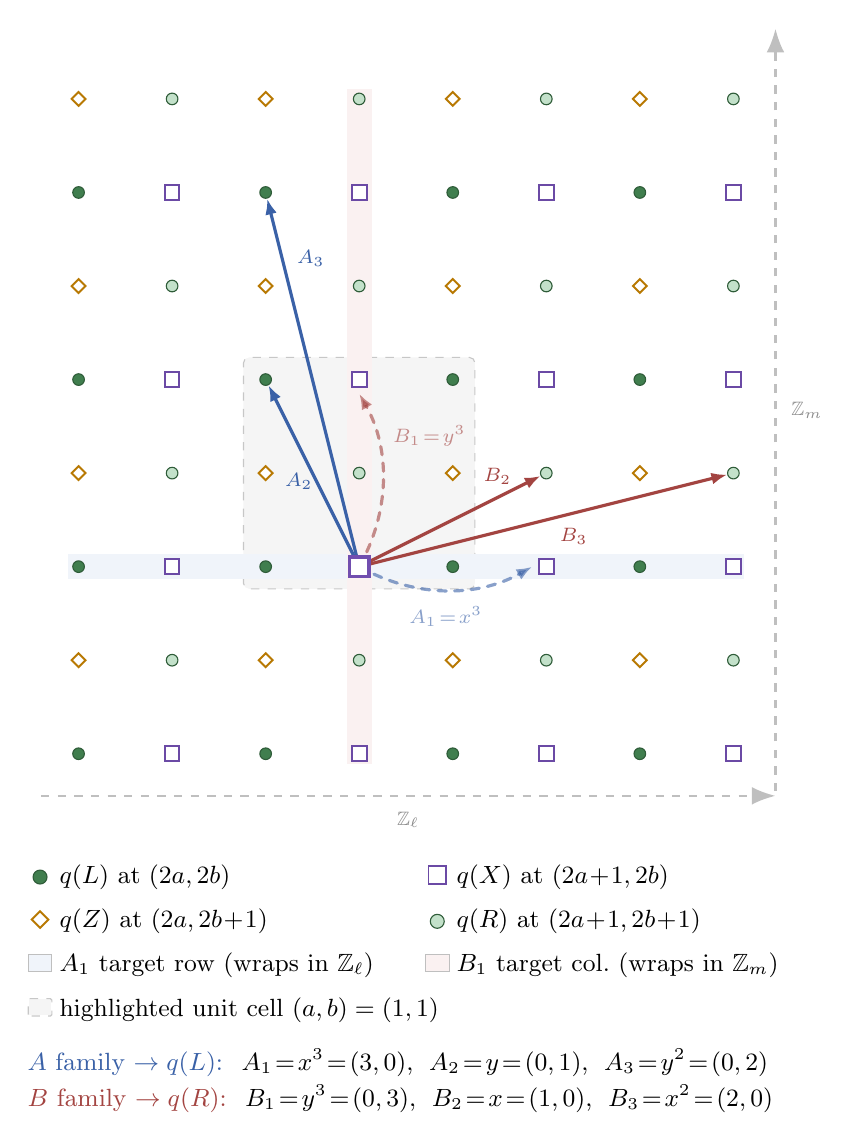
\begin{tikzpicture}[scale=0.88]
  \def\s{1.35}

  % ── Highlighted unit cell (a,b)=(1,1) — fill and border ──
  \fill[black!4, rounded corners=2pt]
    ({2*1*\s-0.32},{2*1*\s-0.32}) rectangle ({(2*1+2)*\s+0.32},{(2*1+2)*\s+0.32});
  \draw[black!22, dashed, rounded corners=2pt]
    ({2*1*\s-0.32},{2*1*\s-0.32}) rectangle ({(2*1+2)*\s+0.32},{(2*1+2)*\s+0.32});

  % ── Wraparound target highlights (clipped to grid extent) ──
  % Grid spans x=[0, (2*3+1)*s], y=[0, (2*3+1)*s].
  % A₁ target row: b=1 (same row, wraps in Z_ℓ). Faint blue stripe.
  \fill[okBlue!8]
    ({-0.15},{2*1*\s-0.18}) rectangle ({(2*3+1)*\s+0.15},{2*1*\s+0.18});
  % B₁ target column: a=1 (same column, wraps in Z_m). Faint red stripe.
  \fill[okRed!8]
    ({(2*1+1)*\s-0.18},{-0.15}) rectangle ({(2*1+1)*\s+0.18},{(2*3+1)*\s+0.15});

  % ── Dashed continuation arrows (drawn BEFORE grid so nodes sit on top) ──
  % A₁ = x³: X(1,1) → q(L,4,1), wraps off-patch to the right.
  % Curved to avoid passing through L(2,1) at (5.40, 2.70).
  \draw[routeA, dashed, opacity=0.60, -{Latex[length=2mm]}]
    ({(2*1+1)*\s},{2*1*\s}) .. controls ++(0.8,-0.45) and ++(-0.8,-0.45) .. ++(1.85*\s,0)
    node[pos=0.50, below=2pt, text=okBlue!85!black, font=\scriptsize] {$A_1\!=\!x^3$};
  % B₁ = y³: X(1,1) → q(R,1,4), wraps off-patch upward.
  % Curved to avoid passing through R(1,1) at (4.05, 4.05).
  \draw[routeB, dashed, opacity=0.60, -{Latex[length=2mm]}]
    ({(2*1+1)*\s},{2*1*\s}) .. controls ++(0.45,0.8) and ++(0.45,-0.8) .. ++(0,1.85*\s)
    node[pos=0.75, right=2pt, text=okRed!85!black, font=\scriptsize] {$B_1\!=\!y^3$};

  % ── Qubit grid: a,b ∈ {0,...,3} ──
  \foreach \a in {0,1,2,3} {
    \foreach \b in {0,1,2,3} {
      \node[qdata] (L\a\b) at ({2*\a*\s},{2*\b*\s}) {};
      \node[qx]    (X\a\b) at ({(2*\a+1)*\s},{2*\b*\s}) {};
      \node[qz]    (Z\a\b) at ({2*\a*\s},{(2*\b+1)*\s}) {};
      \node[qr]    (R\a\b) at ({(2*\a+1)*\s},{(2*\b+1)*\s}) {};
    }
  }

  % ── Tanner-graph edges from X(1,1) (drawn on top of grid) ──
  % A terms → q(L) (solid blue)
  \draw[routeA, -{Latex[length=2mm]}] (X11) -- (L12)
    node[pos=0.65, left=3pt, below=6pt, text=okBlue!85!black, font=\scriptsize] {$A_2$};
  \draw[routeA, -{Latex[length=2mm]}] (X11) -- (L13)
    node[pos=0.85, anchor=west, xshift=2pt, yshift=-2pt, text=okBlue!85!black, font=\scriptsize] {$A_3$};

  % B terms → q(R) (solid red)
  \draw[routeB, -{Latex[length=2mm]}] (X11) -- (R21)
    node[pos=0.75, above=1pt, text=okRed!85!black, font=\scriptsize] {$B_2$};
  \draw[routeB, -{Latex[length=2mm]}] (X11) -- (R31)
    node[pos=0.55, anchor=north, xshift=3pt, yshift=-1pt, text=okRed!85!black, font=\scriptsize] {$B_3$};

  % ── Highlighted X-check (drawn LAST, on top of everything) ──
  \node[qx, draw=okPurple!90!black, fill=white,
        line width=1.25pt, minimum size=7pt] at (X11) {};

  % ── Lattice direction arrows ──
  \draw[black!25, thick, -{Latex[length=3mm]}, dashed]
    ({-0.4*\s},{-0.45*\s}) -- ({(2*3+1)*\s+0.45*\s},{-0.45*\s})
    node[midway, below=2pt, font=\scriptsize, black!45] {$\mathbb{Z}_{\ell}$};
  \draw[black!25, thick, -{Latex[length=3mm]}, dashed]
    ({(2*3+1)*\s+0.45*\s},{-0.4*\s}) -- ({(2*3+1)*\s+0.45*\s},{(2*3+1)*\s+0.75*\s})
    node[midway, right=2pt, font=\scriptsize, black!45] {$\mathbb{Z}_{m}$};

  % ── Coordinate legend (tabular for vertical alignment) ──
  \node[anchor=north west, font=\small, inner sep=0pt]
    at ({-0.55*\s},{-1.15*\s}) {%
    \begin{tabular}{@{}c@{\;}l@{\qquad}c@{\;}l@{}}
      \raisebox{-0.5pt}{\tikz{\node[qdata,scale=1.2] {};}} & $q(L)$ at $(2a,2b)$ &
      \raisebox{-0.5pt}{\tikz{\node[qx,scale=1.2] {};}} & $q(X)$ at $(2a\!+\!1,2b)$ \\[5pt]
      \raisebox{-0.5pt}{\tikz{\node[qz,scale=1.2] {};}} & $q(Z)$ at $(2a,2b\!+\!1)$ &
      \raisebox{-0.5pt}{\tikz{\node[qr,scale=1.2] {};}} & $q(R)$ at $(2a\!+\!1,2b\!+\!1)$ \\[5pt]
      \tikz[baseline=0ex]{\fill[okBlue!8] (0,0) rectangle (0.30,0.22);\draw[black!25,line width=0.3pt] (0,0) rectangle (0.30,0.22);} &
      $A_1$ target row (wraps in $\mathbb{Z}_{\ell}$) &
      \tikz[baseline=0ex]{\fill[okRed!8] (0,0) rectangle (0.30,0.22);\draw[black!25,line width=0.3pt] (0,0) rectangle (0.30,0.22);} &
      $B_1$ target col.\ (wraps in $\mathbb{Z}_{m}$) \\[5pt]
      \tikz[baseline=0ex]{\fill[black!4] (0.01,0.01) rectangle (0.29,0.21);\draw[black!22,dashed,rounded corners=0.5pt] (0,0) rectangle (0.30,0.22);} &
      \multicolumn{3}{@{}l}{highlighted unit cell $(a,b)=(1,1)$}
    \end{tabular}};

  \node[anchor=north west, font=\small, inner sep=0pt]
    at ({-0.55*\s},{-3.15*\s}) {%
    \begin{tabular}{@{}l@{}}
      \textcolor{okBlue!85!black}{$A$ family $\to q(L)$:}\;
      $A_1\!=\!x^3\!=\!(3,0)$,\; $A_2\!=\!y\!=\!(0,1)$,\; $A_3\!=\!y^2\!=\!(0,2)$\\[2pt]
      \textcolor{okRed!85!black}{$B$ family $\to q(R)$:}\;
      $B_1\!=\!y^3\!=\!(0,3)$,\; $B_2\!=\!x\!=\!(1,0)$,\; $B_3\!=\!x^2\!=\!(2,0)$
    \end{tabular}};
\end{tikzpicture}
\end{document}
